\chapter{Folding Automata on the Disk}
\label{chap:folding_automata}

In Chapter \ref{chap:stratoriented}, we successfully eliminated the pseudo-Anosov strata $(2; 1^4, 2^2; \emptyset)$, $(4; 1^6; \emptyset)$, and $(2; 1^6; 4)$ by exploiting the global orientability of their lifted invariant foliations. The remaining possible strata for the disk monodromy---specifically those containing odd-pronged internal singularities, namely $(2; 1^6; 3^2)$ and $(3; 1^6; 3)$---do not admit orientable foliations. To eliminate these final candidates, we cannot rely on the Alexander polynomial. Instead, in Chapter \ref{chap:stratatraintrackanalysis} we will directly construct the valid train track maps within these strata and manually apply the Trace Lemma established in Chapter \ref{chap:train tracks}.

This topological case analysis requires a finite, exhaustive list of candidate standard train tracks to serve as the starting point. While the existence of an invariant train track is guaranteed by the Bestvina-Handel algorithm \cite{bestvina1995train}, we require a systematic enumeration of all possible tracks within our specific strata.

To achieve this, we utilize the concept of the \textit{folding automaton}, introduced by Ko, Los, and Song \cite{SongEntropy}. A folding automaton is a directed graph where vertices represent isomorphism classes of train tracks and edges represent folding operations. For the purposes of this thesis, we utilize the automaton strictly as an \textbf{enumeration engine}. By generating the complete automaton for a given stratum, the set of vertices provides the exact, finite catalog of standard train tracks required for our subsequent analysis.

In this chapter, we describe the theory of folding automata on the $n$-punctured disk $D_n$. We then present our computational implementation of the ``genauto'' algorithm proposed by Ham and Song \cite{HamSong2007}, which we have developed in the software package \texttt{autofolder} to systematically output the candidate tracks for our remaining strata.

\section{Folding and The Folding Automaton}
\label{sec:automaton_definition}

Ko, Los, and Song \cite{SongEntropy} defined the folding automaton $\mathcal{A}_n$ for the braid group $B_n$. This structure encodes all possible standard train tracks (of a fixed complexity) and the transitions between them. First, we must define the procedure of \emph{folding} a train track.

\subsection{Elementary Folding}
\label{subsec:elementary_folding}

To rigorously define the folding operation, we adopt the terminology of Reinoso \cite{reinoso2024pseudo}, who adapts the notion of elementary folding from Ham and Song \cite{HamSong2007}.

\begin{definition}[Markov Map]
    Let $\tau$ and $\tau'$ be standardly embedded train tracks on $D_n$. A \textbf{Markov map} is a graph map $p: \tau \to \tau'$ that maps vertices to vertices and is locally injective away from the preimages of vertices.
\end{definition}

\begin{definition}[Elementary Folding Map]\label{def:elementary_folding_map}
    An \textbf{elementary folding map} is a smooth Markov map $p: \tau \to \tau'$ satisfying the following conditions:
    \begin{enumerate}
        \item \textbf{Edge Lengths:} There exists exactly one real edge $\alpha \in E(\tau)$ such that its image $p(\alpha)$ has word length 2 in the edge basis of $\tau'$. For all other edges $e \in E(\tau) \setminus \{\alpha\}$, the image $p(e)$ has word length 1.
        \item \textbf{Cusp Condition:} The distinguished edge $\alpha$ must belong to a cusp of $\tau$. Specifically, if $\alpha$ and $\beta$ form a cusp at a switch $v$, then $p(\alpha)$ is of the form $p(\beta) \cdot \delta$ (or $\delta \cdot p(\beta)$), effectively ``zipping'' $\alpha$ along $\beta$.
    \end{enumerate}
\end{definition}

In this context, \textit{smoothness} implies that $p$ preserves the tangent structure at the switches, mapping cusps to cusps or smoothing them into arcs, strictly preserving the train track embedding.

The transition matrix $M_p$ of an elementary folding map (with respect to the basis of real edges, in the convention of Section \ref{sec:traintrack_maps}) has a simple structure. All real edges except $\alpha$ map to a single real edge under $p$, contributing a single $1$ to their column. The distinguished edge $\alpha$ maps to a real-edge word of length two, namely $p(\alpha) = p(\beta) \cdot a$ (where $a$ is the real edge joined to $p(\beta)$ by an intermediate infinitesimal edge), contributing a $1$ in the row of $p(\beta)$ and a $1$ in the row of $a$. We may therefore write
\[
M_p = P + E,
\]
where $P$ is a permutation matrix (the column of $\alpha$ assigns it to the destination real edge $a$, and all other columns implement the bijection $p$ acts on the remaining real edges) and $E$ is an elementary matrix --- zero except for a single $1$ in position $(p(\beta), \alpha)$ --- recording the extra traversal of $p(\beta)$ in the image of $\alpha$.

\paragraph{Geometric Description.}
\begin{figure}[h]
    \centering
    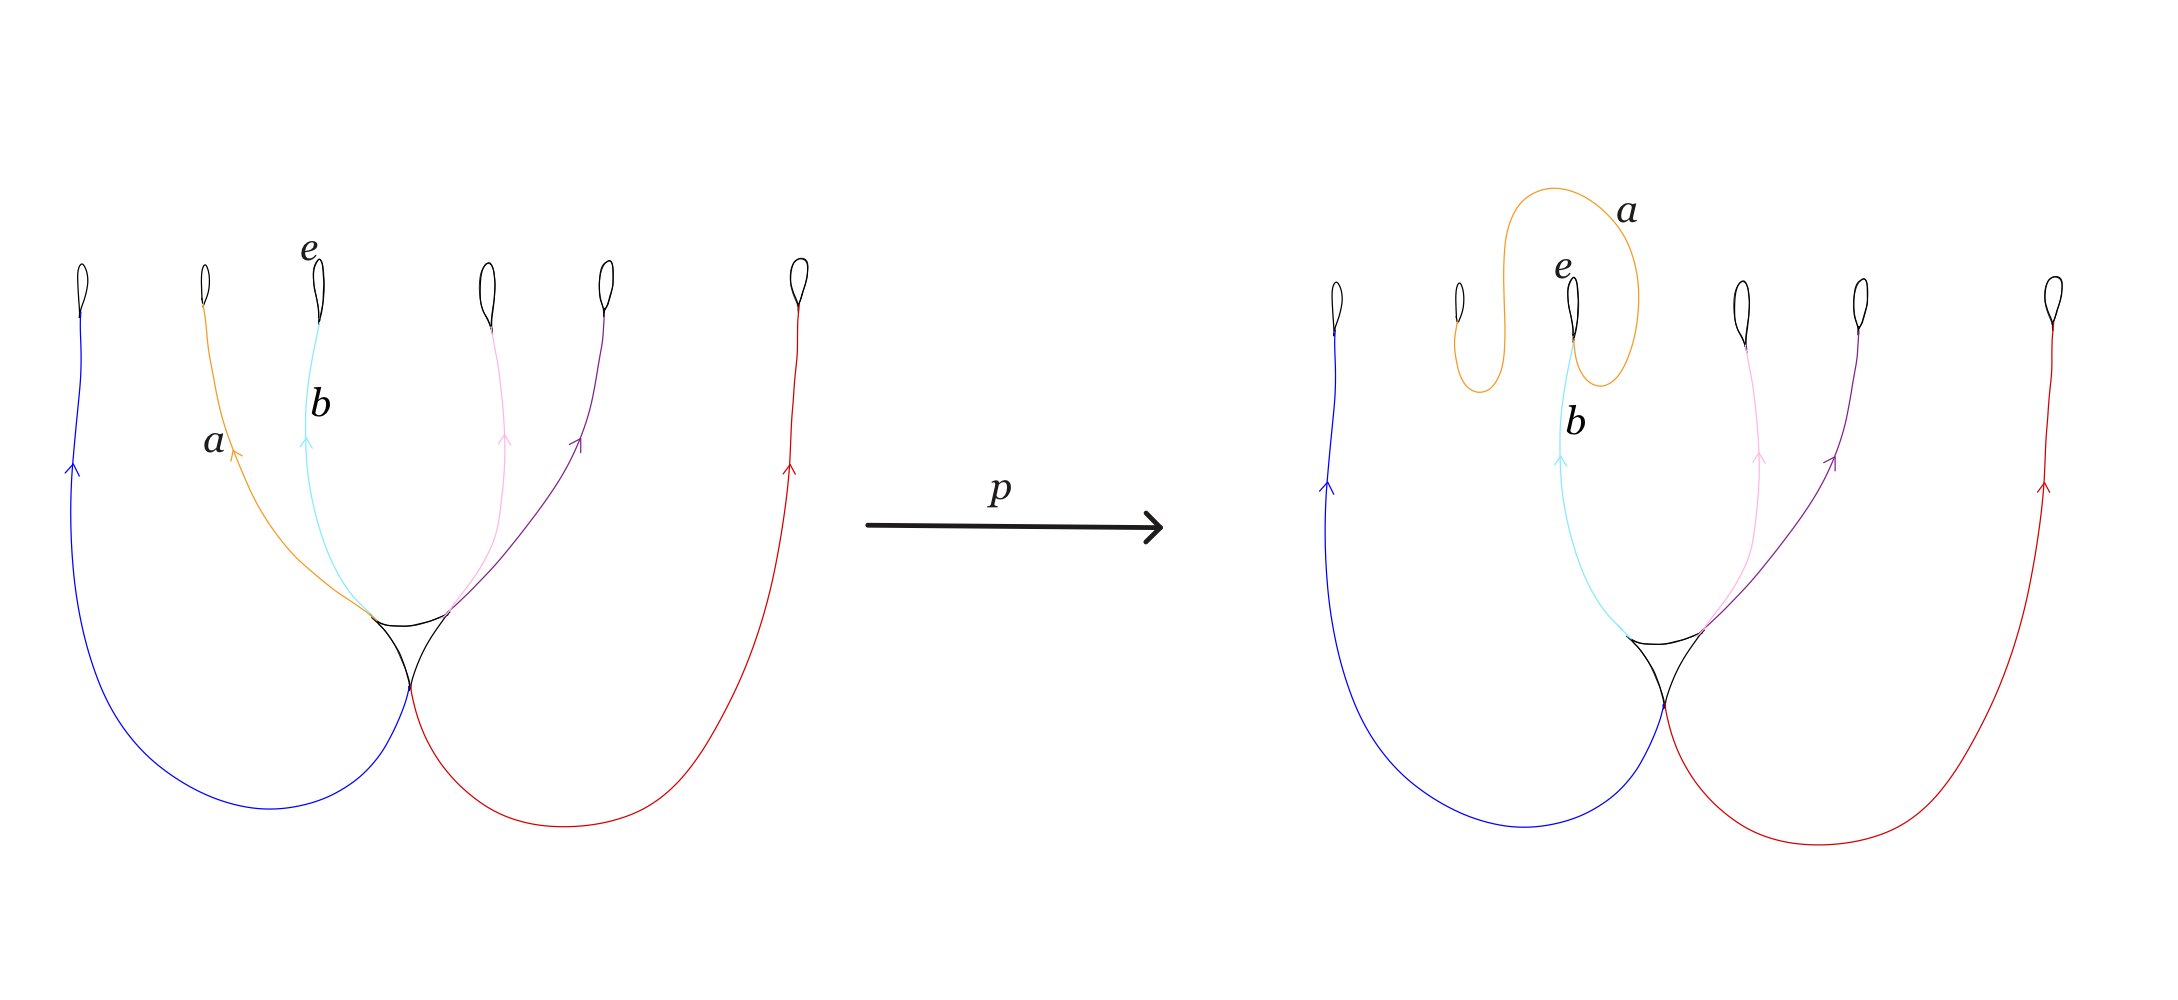
\includegraphics[width=\linewidth]{figures/folding.png}
    \caption{An example of an elementary folding map. The map $p$ is the identity except at the edge $a$, which is mapped as a directed path to $b \cdot e \cdot a$.}
    \label{fig:folding}
\end{figure}

Visually, the folding operation takes place at a \textbf{cusp}---a switch $v$ where two \textit{real} edges, say $a$ and $b$, meet tangentially. In the local cyclic ordering at $v$, these real edges are separated by an infinitesimal edge $e$, which represents the boundary of a punctured region.

To fold $a$ onto $b$, we slide the vertex $v$ along the edge $b$. This action identifies $a$ with a segment of $b$ (``zipping'' them together) and simultaneously drags the endpoint of the edge $a$ along the fold path. The fold terminates when $v$ reaches the vertex at the other end of $e$. At this point, the modified $a$ connects to the infinitesimal edge located at that destination vertex, completing the topological transition. For an example, see Figure \ref{fig:folding}, which shows an elementary folding of $a$ onto $b$ at the cusp formed between the two edges.

\begin{remark}[Why Real Edges?]
    It is important to note that a valid cusp must involve two \textit{real} edges (or at least one real edge, depending on the specific standard definitions used). A cusp formed purely by two infinitesimal edges is forbidden in a standard train track. Dynamically, such a fold would be trivial (mapping zero measure to zero measure). Topologically, two infinitesimal edges meeting at a cusp would imply a singularity on the boundary of a puncture that is not connected to the interior foliation; such a configuration is unstable and can be removed by isotopy.
\end{remark}

\subsection{The Standardizing Braid}
\label{subsec:standardizing_braid}

While an elementary folding map $p: \tau \to \tau'$ preserves the foliation data, the resulting graph $\tau'$ often fails to satisfy the vertical marking condition of a standard train track. For example, the folding operation in Figure \ref{fig:folding} produces a non-standard train track. Recall from Definition \ref{def:standard_track}, the vertical marking condition requires that for each marked point, there is exactly one infinitesimal edge of $\tau$ passing vertically above it. In practice, this infinitesimal edge belongs to the infinitesimal polygon surrounding the marked point.

After an elementary fold starting from a standard train track $\tau$, the folded track $\tau'$ often violates the vertical marking condition; however, Ko-Los-Song \cite{SongEntropy} show that $\tau'$ is at most \emph{almost standard}. That is, $\tau'$ has at most one offending infinitesimal edge. In other words, there is at most one marked point having two infinitesimal edges lying above it. We can perform a homeomorphism of the disk to transform the embedding of the folded train track so that it becomes standard. This choice of homeomorphism fixes the boundary pointwise, is orientation-preserving, and respects the marked points (permutes them), and thus can be thought of as a braid. We call such a braid a \textit{standardizing braid}. This standardizing braid is non-unique for a given almost standard train track. However, it can be taken to be of a certain form\footnote{Recall that braid words are read from left to right.}:

\begin{lemma}[{\cite[Lemma~1]{SongEntropy}}]
    Let $\tau'$ be an almost standard train track on $D_n$. Then there exists an $n$-braid $\beta \in B_n$ of the form
    \[
    \beta = \delta_{[l,m]}^{\pm 1},
    \]
    where
    \[
    \delta_{[l,m]} = \sigma_{m-1}\sigma_{m-2}\cdots \sigma_{l},
    \]
    is the $n$-braid written in standard Artin generators, so that $\beta (\tau')$ is a standard train track on $D_n$.
\end{lemma}

Figure \ref{fig:standardizing} shows an example of a standardizing operation following an elementary fold.

\begin{figure}[h]
    \centering
    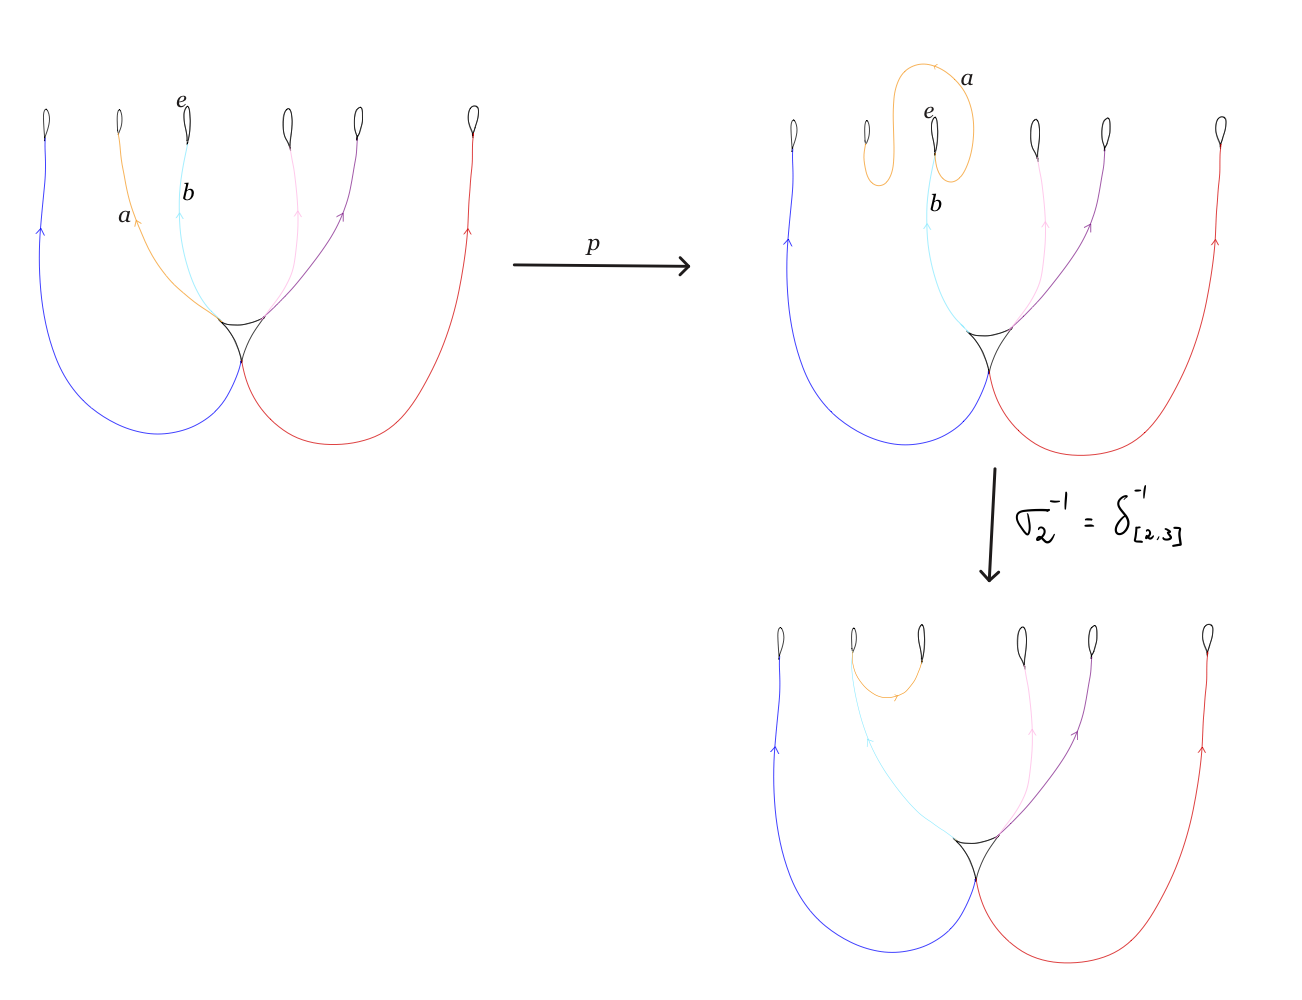
\includegraphics[width=\linewidth]{figures/standardizing.png}
    \caption{The braid $\delta_{[2,3]}^{-1} = \sigma_2^{-1}$ standardizes the folded train track.}
    \label{fig:standardizing}
\end{figure}

\subsection{The Folding Automaton}
A pseudo-Anosov braid $\beta$ induces a train track map $f_\beta: \tau \to \tau$ on a standard train track $\tau$. By the work of Bestvina-Handel and others, $f_\beta$ admits a decomposition into a sequence of elementary folding maps followed by a train track isomorphism:
\begin{equation}\label{equation:folding_decomposition}
        f_\beta \simeq \psi \circ p_k \circ \dots \circ p_1,
\end{equation}
where each $p_i: \tau_{i-1} \to \tau_i$ is an elementary folding map and $\psi: \tau_k \to \tau_0$ is an isomorphism, that is, a train track map induced by an orientation-preserving pointed homeomorphism of the disk.

It is further shown that the folding decomposition of Equation \eqref{equation:folding_decomposition} can be rewritten so that it implies that the braid $\beta$ decomposes as the composition of standardizing braids associated to the elementary folding operations $p_i$, along with a braid inducing the isomorphism $\psi$:

\begin{equation}\label{equation:folding_decomposition_braid}
    \beta = \Delta_n^{2m} \Psi \circ \beta_{p_k} \circ \dots \circ \beta_{p_1}.
\end{equation}

Here $\Psi$ is a braid inducing the train track isomorphism $\psi \colon \tau_k \to \tau_0$; the term $\Delta_n^{2m}$ accounts for an ambiguity arising from the Dehn twists along the outer boundary. This motivates the following definition:

\begin{definition}
    Let $\tau$ and $\tau'$ be train tracks on $D_n$ (not necessarily standard). We say $\tau$ and $\tau'$ are \emph{isomorphic} if there exists a braid inducing a train track isomorphism between the two train tracks.
\end{definition}

Geometrically, this definition is equivalent to saying that $\tau$ and $\tau'$ are ambient isotopic relative to the boundary, via an isotopy that is permitted to permute the marked points.

We are now ready to give the formal definition of the folding automaton:

\begin{definition}[Folding Automaton]
    The folding automaton $\mathcal{A}$ is a directed graph defined as follows:
    \begin{itemize}
        \item \textbf{Vertices:} The set of vertices $V(\mathcal{A})$ consists of isomorphism classes of standard train tracks on $D_n$. In other words, each vertex represents an orbit of standard tracks under the action of the braid group $B_n$.
        \item \textbf{Edges:} A directed edge exists from a class $[\tau_1]$ to $[\tau_2]$ if there exists a standard train track $\tau \in [\tau_1]$ and a valid cusp $c$ such that folding $\tau$ at $c$ and standardizing yields a track $\tau' \in [\tau_2]$.
        \item \textbf{Labels:} The directed edge is labeled by the standardizing braid $\beta_{std} \in B_n$ required to return the folded track to standard form.
    \end{itemize}
\end{definition}

\paragraph{Stratum Specificity}
It is important to emphasize that in our context, an automaton is constructed for a \textbf{single, fixed stratum} of the space of measured foliations $\mathcal{PMF}(D_n)$. The stratum is determined by the number and type of singularities of the foliations carried by the tracks. This restriction to a single stratum is a natural consequence of the folding operation itself. Geometrically, the complementary regions of a standard train track correspond precisely to the singularities of the measured foliations it carries; the cusps along the boundary of each complementary region count the prongs of the corresponding singularity (Proposition \ref{prop:B-H train track polygon enclosure}). An elementary folding map modifies the embedding of $\tau$ only locally near the folded edge $\alpha$, replacing $\alpha$ with a path that forms a bigon with the original edge inside its enclosing complementary region. This local modification fixes the boundary of every complementary region setwise and preserves the cusp count along each boundary. Therefore folding leaves the singularity stratum invariant: if a track $\tau$ decomposes the disk into a specific configuration of $k$-gons, every track reachable from $\tau$ via folding decomposes the disk into exactly the same set of $k$-gons.

\begin{corollary}
    Let $(\beta, \phi_\beta, \tau, f_\beta)$ be geometric data of a pseudo-Anosov $n$-braid. Then $\tau$ appears as a vertex in the folding automaton associated to the particular stratum $\phi_\beta$ belongs to.
\end{corollary}

\begin{corollary}
    Let $\beta$ be a pseudo-Anosov $n$-braid. Up to conjugacy, a decomposition of $\beta$ in the form of Equation \eqref{equation:folding_decomposition_braid} appears as a cycle in the folding automaton.
\end{corollary}
\begin{myproof}
    By Proposition \ref{prop:every_pA_carried_by_standard_track}, $\beta$ is carried by a standard train track $\tau$, and the isomorphism class of $\tau$ must exist as a vertex in the folding automaton.
\end{myproof}

Figure \ref{fig:automaton} shows an example of a folding automaton of the 4-marked disk, on the stratum $(1;1^4;1)$. The solid lines represent folding operations, where ``ROL fold'' means \textbf{Right-Over-Left fold}. This indicates that the edge on the right-hand side of the cusp (facing toward the mouth of the cusp) is folded over the edge on the left-hand side. Since there is a single cusp in this example, this is sufficient to specify the particular folding operation. The analogous \textbf{Left-Over-Right Fold} is represented by ``LOR fold''.

The dotted lines are standardizing operations and thus represent isomorphisms. Consequently, this specific automaton is a directed graph with three vertices and six directed edges.

\begin{figure}[h]
    \centering
    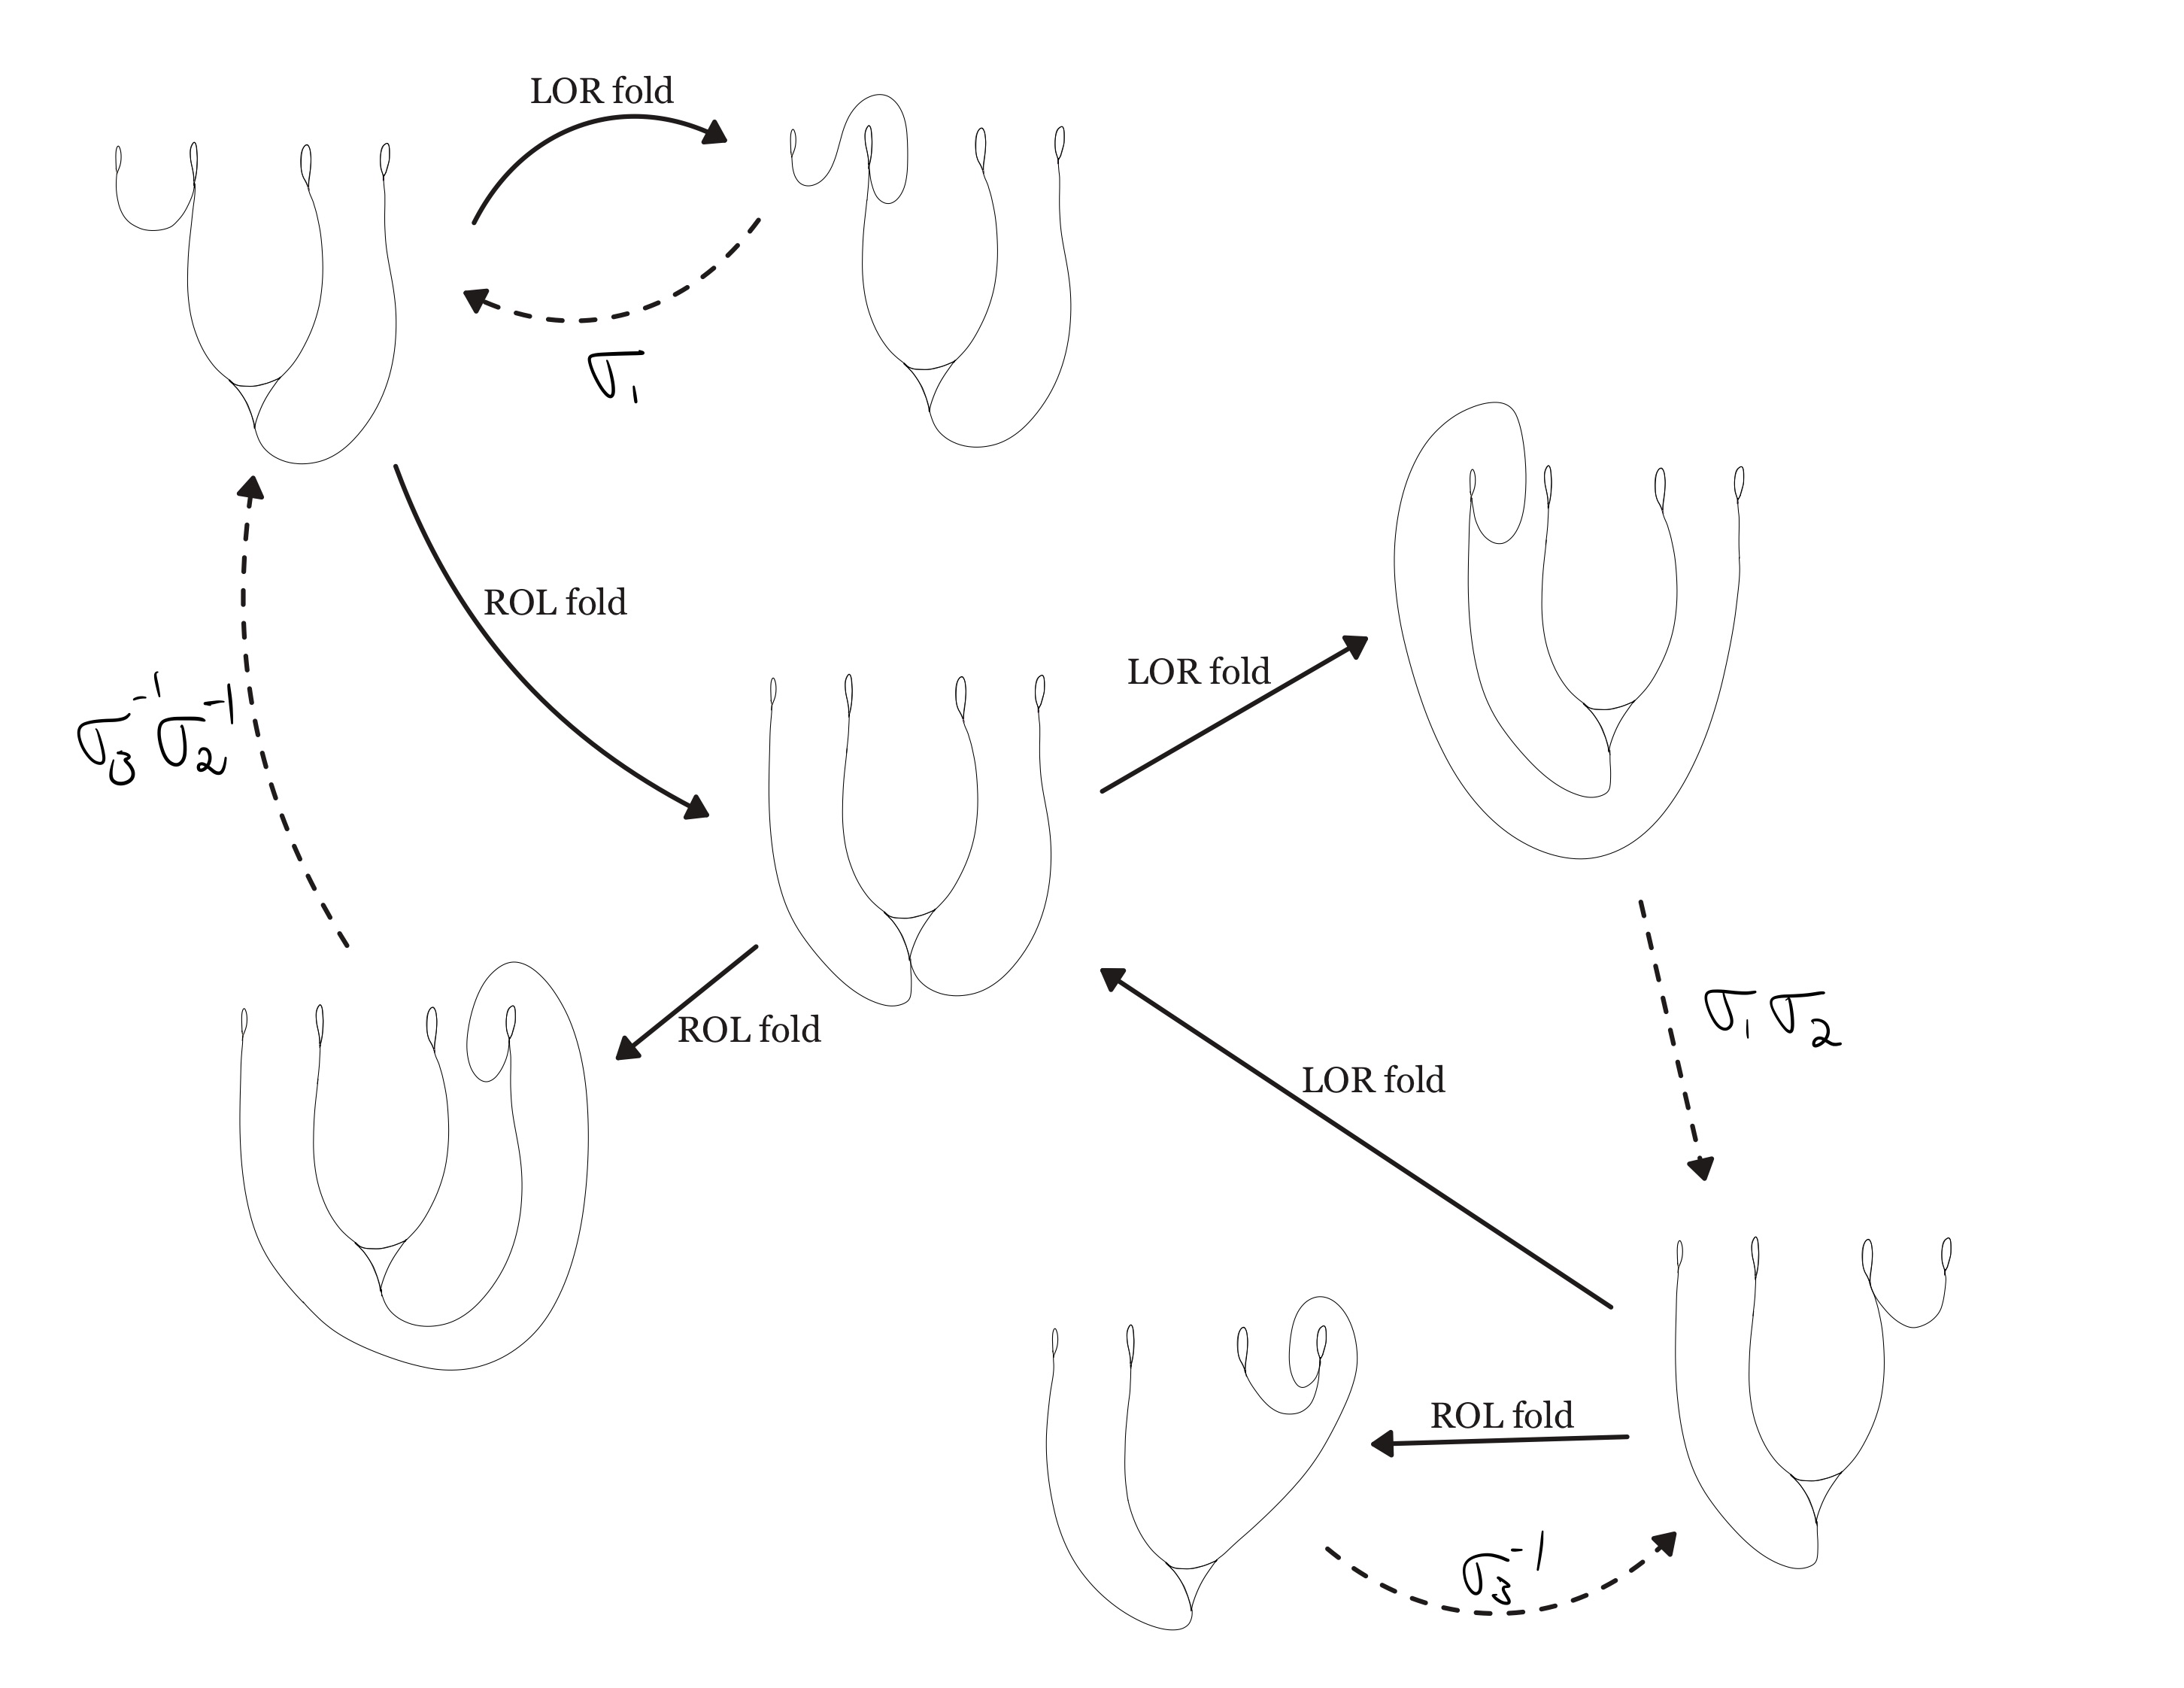
\includegraphics[width=\linewidth]{figures/Automaton.jpg}
    \caption{The folding automaton of the stratum $(1;1^4;1)$ on the 4-marked disk.}
    \label{fig:automaton}
\end{figure}

In general, the folding automaton of a particular stratum can become extremely complicated as soon as the disk under consideration has 5 or 6 marked points, making it impracticable to reproduce graphically.

Ham and Song \cite{HamSong2007} proposed an algorithm for generating the folding automaton, which they termed \texttt{genauto}. The theoretical version of this algorithm, as described in the appendix of their work, is presented below. It requires a ``seed'' standard train track belonging to the stratum of interest. That is, suppose we would like to generate the folding automaton of the stratum
\[
(b_1,\dots,b_r; m_1,\dots, m_n ; k_1,\dots, k_s),
\]
then we must choose a seed standard train track $\tau$ whose peripheral region $D_n \setminus \tau$ is an $r$-gon; whose $i$th marked point is enclosed by an $m_i$-gon; and whose $i$th non-marked polygon is $k_i$-sided. The algorithm will then proceed to identify all of the cusps available to perform folding operations. Each time it performs a folding operation and obtains a new train track, it checks against the list of current train tracks (which initializes to a set only containing $\tau$). If it finds it in the list, a directed edge is created pointing to it, and the edge is decorated by a standardizing braid. If it does not find it in the list, the new train track is added to the list, with a directed edge pointing to it, again decorated with a standardizing braid. The algorithm exhausts every possible folding operation on every train track in the list.

\begin{algorithm}[H]
\caption{genauto (Theoretical \cite{HamSong2007})}
\label{alg:genauto_theoretical}
\begin{algorithmic}[1]
\State Let $S$ be a set of standard train tracks, initialized with a seed track: $S \gets \{ \tau_{seed} \}$.
\State Let $N$ be the set of new tracks found in the current iteration.
\Repeat
    \State $N \gets \emptyset$
    \For{every track $\tau \in S$}
        \For{every valid cusp $c$ in $\tau$}
            \State $\tau' \gets \text{Fold}(\tau, c)$
            \State $\tau_{std} \gets \text{Standardize}(\tau')$
            \If{$\tau_{std}$ is not isomorphic to any track in $S$}
                \State $N \gets N \cup \{ \tau_{std} \}$
            \EndIf
        \EndFor
    \EndFor
    \State $S \gets S \cup N$
\Until{$N = \emptyset$}
\State \Return The graph with vertices $S$ and edges determined by the folds.
\end{algorithmic}
\end{algorithm}

\subsection{Proof of Completeness and Termination}
\label{sec:autofolder_proof}

In the Introduction, we stated Theorem \ref{thm:autofolder_main}, asserting that the algorithmic realization of the folding automaton provides a complete and finite classification of all standard train tracks for a given stratum. The proof has two parts: \textit{exhaustiveness} (the algorithm visits every isomorphism class of standard tracks in the stratum) and \textit{finiteness} (the algorithm terminates). Exhaustiveness rests on a connectivity theorem of Penner and Harer; finiteness rests on a counting bound for standard tracks on the punctured disk.

\begin{theorem}[Completeness of the \texttt{genauto} algorithm]
\label{thm:genauto_completeness}
    Let $\mathcal{S}$ be a connected stratum of the space of measured foliations on $D_n$. Given a seed standard train track $\tau_{seed} \in \mathcal{S}$, the \texttt{genauto} algorithm terminates and returns the complete, finite list of isomorphism classes of standard train tracks in $\mathcal{S}$.
\end{theorem}

\begin{myproof}
\textbf{Exhaustiveness.}
The exhaustiveness argument relies on a connectivity result of Penner and Harer phrased in terms of \emph{splitting}, the topological inverse of folding. We will define splitting more carefully and use it heavily in Chapter \ref{chap:stratatraintrackanalysis}; for the present proof, it suffices to know that a split is a local move on a train track that reverses an elementary fold --- if a track $\tau$ folds to $\tau'$, then $\tau'$ splits to $\tau$. A split is permitted at a switch where the local geometry admits an inverse-fold configuration; not every switch can be split, but every fold can be undone by a split.

With this, we may state the relevant Penner-Harer connectivity result \cite{penner1992combinatorics}: the space of measured laminations $\mathcal{ML}_0(D_n)$ admits a cellular decomposition whose cells correspond to standard train tracks, and any two equivalent positively measured standard tracks $(\tau_1, \mu_1)$ and $(\tau_2, \mu_2)$ admit a common refinement $(\tau, \mu)$, in the sense that each $(\tau_i, \mu_i)$ splits (and isotopes) to $(\tau, \mu)$ \cite[Theorem~2.3.1]{penner1992combinatorics}. Consequently, any two standard tracks in the same stratum are related by a finite sequence of splits and inverse splits (i.e., folds) modulo isotopy.

To translate this geometric statement into the combinatorial language of folding automata:
\begin{itemize}
    \item \textbf{Splitting is inverse folding:} As stated above, splitting and folding are mutually inverse local moves. A splitting move corresponds to traversing a directed edge of the automaton backwards.
    \item \textbf{Connectivity of the automaton:} Since any two tracks in the stratum are related by a sequence of splits and folds, the folding automaton is connected as an \emph{undirected} graph.
\end{itemize}

The \texttt{genauto} algorithm performs a breadth-first search on the directed automaton starting from $\tau_{seed}$. Because the underlying undirected graph is connected, every vertex is reachable from $\tau_{seed}$ by some directed path: any sequence of splits and folds connecting $\tau_{seed}$ to a target $\tau'$ may be rewritten as a sequence of folds (possibly through intermediate vertices not on the shortest path). Hence the BFS exhausts every isomorphism class of standard tracks in the stratum.

\textbf{Finiteness.}
A standard train track on the $n$-marked disk is a finite graph $G$ whose switches have valence at least $3$ (Definition \ref{def:train_track_general}), and whose vertex and edge counts are bounded by the stratum's singularity data via the Euler-Poincar\'{e} formula. The number of switches and real edges admits a uniform bound depending only on $n$ and the singularity profile (specifically, the sum of cusp counts $\sum b_i + \sum m_j + \sum k_l$, which determines the total switch valence and hence both the switch and edge counts up to the polygon structure). The cyclic ordering at each switch admits only finitely many configurations, and only finitely many labelings of edges as real or infinitesimal are compatible with a given polygon structure. Therefore the set of isomorphism classes of standard tracks in a fixed stratum is finite.

The algorithm checks each newly generated track against the registry of previously discovered isomorphism classes (Algorithm \ref{alg:autofolder_enum}). If a fold yields an isomorphism class already in the registry, it is not enqueued for further exploration. Since the state space is finite, the BFS frontier must eventually empty, and the algorithm terminates.

Combining the two parts, the algorithm produces a finite, exhaustive enumeration of the standard tracks in the stratum.
\end{myproof}

\section{Computational Implementation: \texttt{autofolder}}
\label{sec:implementation}
The relevance of folding automata to our work on the detection of the connect-sum of trefoils lies in our analysis of the non-orientable strata $(3;1^6;3)$ and $(2;1^6;3^2)$ on $D_6$. Specifically, having an implementation of the \texttt{genauto} algorithm will allow us to generate all possible isomorphism classes of standard train tracks $[\tau]$ that may fit into geometric data $(\beta, \phi_\beta, \tau, f_\beta)$ belonging to those strata.

To that end, we implemented a robust version of the \texttt{genauto} algorithm in Python. Our software, \texttt{autofolder}, constructs the folding automaton for specified strata on the punctured disk. The implementation handles the complexities of graph isomorphism and explicit folding mechanics.

\subsection{Combinatorial Structure and Equivalence}
\label{subsec:comb_iso}

When the algorithm generates a new track (Algorithm \ref{alg:autofolder_enum}, Line 9), it must determine if this track corresponds to a state already existing in the automaton. To perform this check algorithmically, we rely on the discrete data of the graph structure.

\begin{definition}[Combinatorial Structure]
    The \textit{combinatorial structure} of a train track $\tau$ is the tuple $\mathcal{C}(\tau) = (G, \mathcal{O}, \ell)$, where:
    \begin{itemize}
        \item $G = (V, E)$ is the underlying graph.
        \item $\mathcal{O} = \{ \sigma_v : v \in V \}$ is the set of cyclic permutations recording the counter-clockwise ordering of edges at each switch.
        \item $\ell: E \to \{ \text{real, infinitesimal} \}$ is the labeling function distinguishing edge types.
    \end{itemize}
\end{definition}

\begin{definition}[Combinatorial Equivalence]
    Let $\tau$ and $\tau'$ be two train tracks with combinatorial structures $\mathcal{C}(\tau) = (G, \mathcal{O}, \ell)$ and $\mathcal{C}(\tau') = (G', \mathcal{O}', \ell')$.

    We say that $\tau$ and $\tau'$ are \textbf{combinatorially equivalent} if there exists a graph isomorphism $\phi: G \to G'$ satisfying:
    \begin{enumerate}
        \item \textbf{Structure Preserving:} The isomorphism $\phi$ respects the cyclic ordering of edges at every vertex. That is, for every vertex $v \in V(G), $ the cyclic permutation at the image vertex $\phi(v)$ is the conjugation of the permutation at $v$ by $\phi$:
        \[
            \sigma'_{\phi(v)} = \phi \circ \sigma_v \circ \phi^{-1}
        \]
        \item \textbf{Label Preserving:} The isomorphism $\phi$ respects the edge labelings:
        \[
            \ell'(\phi(e)) = \ell(e) \quad \text{for all } e \in E(G).
        \]
    \end{enumerate}
    In this case, we write $\mathcal{C}(\tau) \cong \mathcal{C}(\tau')$ and say that the train tracks define the same combinatorial state.
\end{definition}

We now prove that checking combinatorial equivalence is sufficient to establish train track isomorphism, thereby providing a rigorous method for state detection in the \texttt{genauto} algorithm.

\begin{prop}
    \label{prop:comb_iso}
    Let $\tau_1$ and $\tau_2$ be standard train tracks on $D_n$. Then $\tau_1$ and $\tau_2$ are isomorphic (i.e., differ by a braid) if and only if they are combinatorially equivalent.
\end{prop}

\begin{myproof}
    $(\Rightarrow)$ Suppose $\tau_1$ and $\tau_2$ are isomorphic. By definition, there exists an orientation-preserving diffeomorphism $h: D_n \to D_n$ (representing a braid $\beta$) such that $h(\tau_1)$ is isotopic to $\tau_2$. Since $h$ is a diffeomorphism, it induces a graph isomorphism $\phi = h|_{\tau_1}: \tau_1 \to \tau_2$. Because $h$ is orientation-preserving, it strictly respects the cyclic ordering of edges at every vertex. Furthermore, as an isomorphism of train tracks, $h$ maps real edges to real edges and infinitesimal edges to infinitesimal edges. Thus, $\phi$ is a combinatorial equivalence and $\mathcal{C}(\tau_1) \cong \mathcal{C}(\tau_2)$.

    $(\Leftarrow)$ Suppose $\phi: \mathcal{C}(\tau_1) \to \mathcal{C}(\tau_2)$ is a combinatorial equivalence. We construct the required braid $\beta$ in three steps.

    \textbf{Step 1: Constructing a homeomorphism between fibered neighborhoods.}
    The tuple $(G, \mathcal{O})$ defines a unique ribbon graph structure. Following Penner and Harer \cite[Section 1.1]{penner1992combinatorics}, this combinatorial data uniquely determines an oriented surface with boundary $N(\tau_i)$ obtained by thickening the ribbon graph; in our setting, $N(\tau_i)$ is the fibered neighborhood of $\tau_i$. Since $\phi$ preserves the cyclic ordering $\mathcal{O}$, it induces an orientation-preserving homeomorphism $h': N(\tau_1) \to N(\tau_2)$ that carries $\tau_1$ onto $\tau_2$ and respects the vertical-fiber structure.

    \textbf{Step 2: Extending across the complementary regions.}
    The complement $D_n \setminus N(\tau_i)$ is a disjoint union of polygons: marked infinitesimal polygons (containing one marked point each), unmarked infinitesimal polygons (containing one non-marked singularity each), and a single peripheral region (adjacent to $\partial D_n$). The combinatorial equivalence $\phi$ induces a bijection between these polygons preserving cusp counts and edge labels, so it sends each polygon of $\tau_1$ to a polygon of $\tau_2$ of the same combinatorial type. We extend $h'$ across each polygon by the Alexander trick (any orientation-preserving homeomorphism of the boundary of a disk extends to a homeomorphism of the disk; the extension is unique up to isotopy rel boundary).

    \emph{Marked polygons.} For a marked $k$-gon enclosing the marked point $q_i \in \tau_1$, the boundary map specified by $h'$ extends to a homeomorphism sending $q_i$ to the corresponding marked point $q_{\phi(i)} \in \tau_2$ (since the vertical infinitesimal edge above each marked point is preserved by $\phi$, the marked point is determined by the polygon structure).

    \emph{Peripheral region.} For the peripheral region $P$ (adjacent to $\partial D_n$), the boundary $\partial P$ consists of $\partial D_n$ together with a portion of $\tau_i$. We choose the Alexander-trick extension on $P$ to be the identity on $\partial D_n$. This is permissible because $\partial D_n \subset \partial P$ is one of the boundary components of $P$, and the Alexander extension is free to be the identity on any single boundary component.

    The composite map $h: D_n \to D_n$ is an orientation-preserving homeomorphism, satisfying $h(\tau_1) = \tau_2$ as embedded subsets of $D_n$, fixing $\partial D_n$ pointwise, and permuting the marked points.

    \textbf{Step 3: Defining the braid.}
    Since $h$ is an orientation-preserving homeomorphism of $D_n$ fixing $\partial D_n$ pointwise and permuting the marked points, it represents an element $\beta = [h] \in \mathrm{Mod}(D_n) \cong B_n$. The action of $\beta$ on isotopy classes of embedded subsets of $D_n$ sends $[\tau_1]$ to $[h(\tau_1)] = [\tau_2]$. That is, $\beta(\tau_1)$ is isotopic to $\tau_2$ as embedded train tracks, so $\tau_1$ and $\tau_2$ are isomorphic in the sense of the chapter.
\end{myproof}

\subsection{Data Structures}
\label{subsec:data_structures}

To implement the \texttt{genauto} algorithm, we must encode the combinatorial structure of the tracks and the auxiliary data required for the folding operations.

The core data structure in our software is the \texttt{StandardTrainTrack} class, which inherits from a base \texttt{TrainTrack} class. This class encodes the train track $\tau$ combinatorially as a decorated graph structure $\mathcal{C}(\tau) = (G, \mathcal{O}, \ell)$ along with embedding data:
\begin{itemize}
    \item \textbf{Graph Representation (\texttt{graph}):} The underlying graph $G$ is stored using the SageMath \texttt{Graph} class, which provides optimized methods for standard graph invariants.
    \item \textbf{Cyclic Ordering (\texttt{vert\_orders}):} A dictionary representing $\mathcal{O}$, mapping each vertex $v$ to the counter-clockwise list of its incident edges. This encodes the ribbon graph structure required to define the surface.
    \item \textbf{Singularity Data (\texttt{infpoly}):} The labeling function $\ell$ is encoded via the \texttt{infpoly} dictionary, which lists the sequences of vertices bounding each infinitesimal polygon (puncture). Edges connecting consecutive vertices in these lists are identified as \textit{infinitesimal}, while all other edges are \textit{real}.
    \item \textbf{Cusp Information (\texttt{cusps}):} A list of \texttt{cusp} objects, enabling the \texttt{fold} method to iterate efficiently over valid folding sites.
\end{itemize}

\subsection{Implementation of Detecting Combinatorial Equivalence}
A significant challenge in generating the automaton is detecting when two distinct \texttt{StandardTrainTrack} objects represent the same vertex in the automaton. Recall that vertices correspond to tracks equivalent up to the action of the braid group. In our implementation, this check is performed by the method \texttt{is\_isomorphic\_to}:

\begin{itemize}
    \item \textbf{Graph Isomorphism Check:} The function first verifies if the underlying graphs are isomorphic using computationally cheap invariants (vertex and edge counts) and the SageMath \texttt{is\_isomorphic} method.
    \item \textbf{Permutation Search (The Braid Action):} If the underlying graphs match, the algorithm must verify if the cyclic orderings and singularity data can be aligned. Crucially, to account for the action of the braid group (which acts by permuting the marked points), the algorithm iterates through all valid permutations of the singularity types. It returns \texttt{True} if there exists a permutation $\sigma$ of the polygons such that relabeling the graph according to $\sigma$ yields a match in both the adjacency structure and the cyclic ordering $\mathcal{O}$.
\end{itemize}

\subsection{Implementation of the Folding Operation}
\label{subsec:folding_implementation}

The engine of the automaton generation is the \texttt{fold} method. It transforms the combinatorial structure of a track $\tau$ into a new track $\tau'$ according to the topological definition of an elementary fold. It takes as input a specific cusp object $c$ and a direction $d \in \{0, 1\}$ (representing Right-over-Left or Left-over-Right).

The procedure executes the following algorithmic steps, modifying the track data in place:

\begin{enumerate}
    \item \textbf{Cusp and Edge Identification:}
    The algorithm first retrieves the local geometry of the cusp $c$. Let $v_{cusp}$ be the cusp vertex, and let $e_L, e_R$ be the incident left and right real edges connecting $v_{cusp}$ to vertices $v_L$ and $v_R$, respectively.
    Based on the folding direction $d$, we identify an \textit{intermediate vertex} $v_{int}$ and the specific \textit{infinitesimal edge} $e_{inf}$ that the fold will traverse.
    Before proceeding, the method validates that $e_{inf}$ is indeed an infinitesimal edge. If $e_{inf}$ is a real edge, the fold is illegal, and the operation returns failure.

    \item \textbf{Graph Surgery (Topological Transition):}
    The folding operation is realized combinatorially by ``zipping'' one branch of the cusp along the infinitesimal edge. Let $v_{far}$ be the vertex at the other end of $e_{inf}$. The algorithm updates the graph $G$ by essentially moving the endpoint of the folded edge from $v_{int}$ to $v_{far}$. This rewiring corresponds to the topological quotient map where the infinitesimal interval $e_{inf}$ is collapsed into the train track.

    \item \textbf{Updating Cyclic Orderings:}
    The algorithm modifies the ribbon structure $\mathcal{O}$ to reflect the new embedding. The new edge must be inserted into the cyclic order $\mathcal{O}_{v_{far}}$ immediately adjacent to $e_{inf}$, preserving the planar embedding. At the folded vertex, the old edge is removed from the ordering, and the new edge is inserted in its place.

    \item \textbf{Cusp Evolution:}
    Finally, the algorithm updates the list of cusps for the new track. The folding operation destroys the original cusp $c$ and creates a new cusp at $v_{far}$.
\end{enumerate}

The method returns a mutated \texttt{StandardTrainTrack} object representing the folded track.

See Figure \ref{fig:folding_automaton} for an example.

\begin{figure}[H]
    \centering
    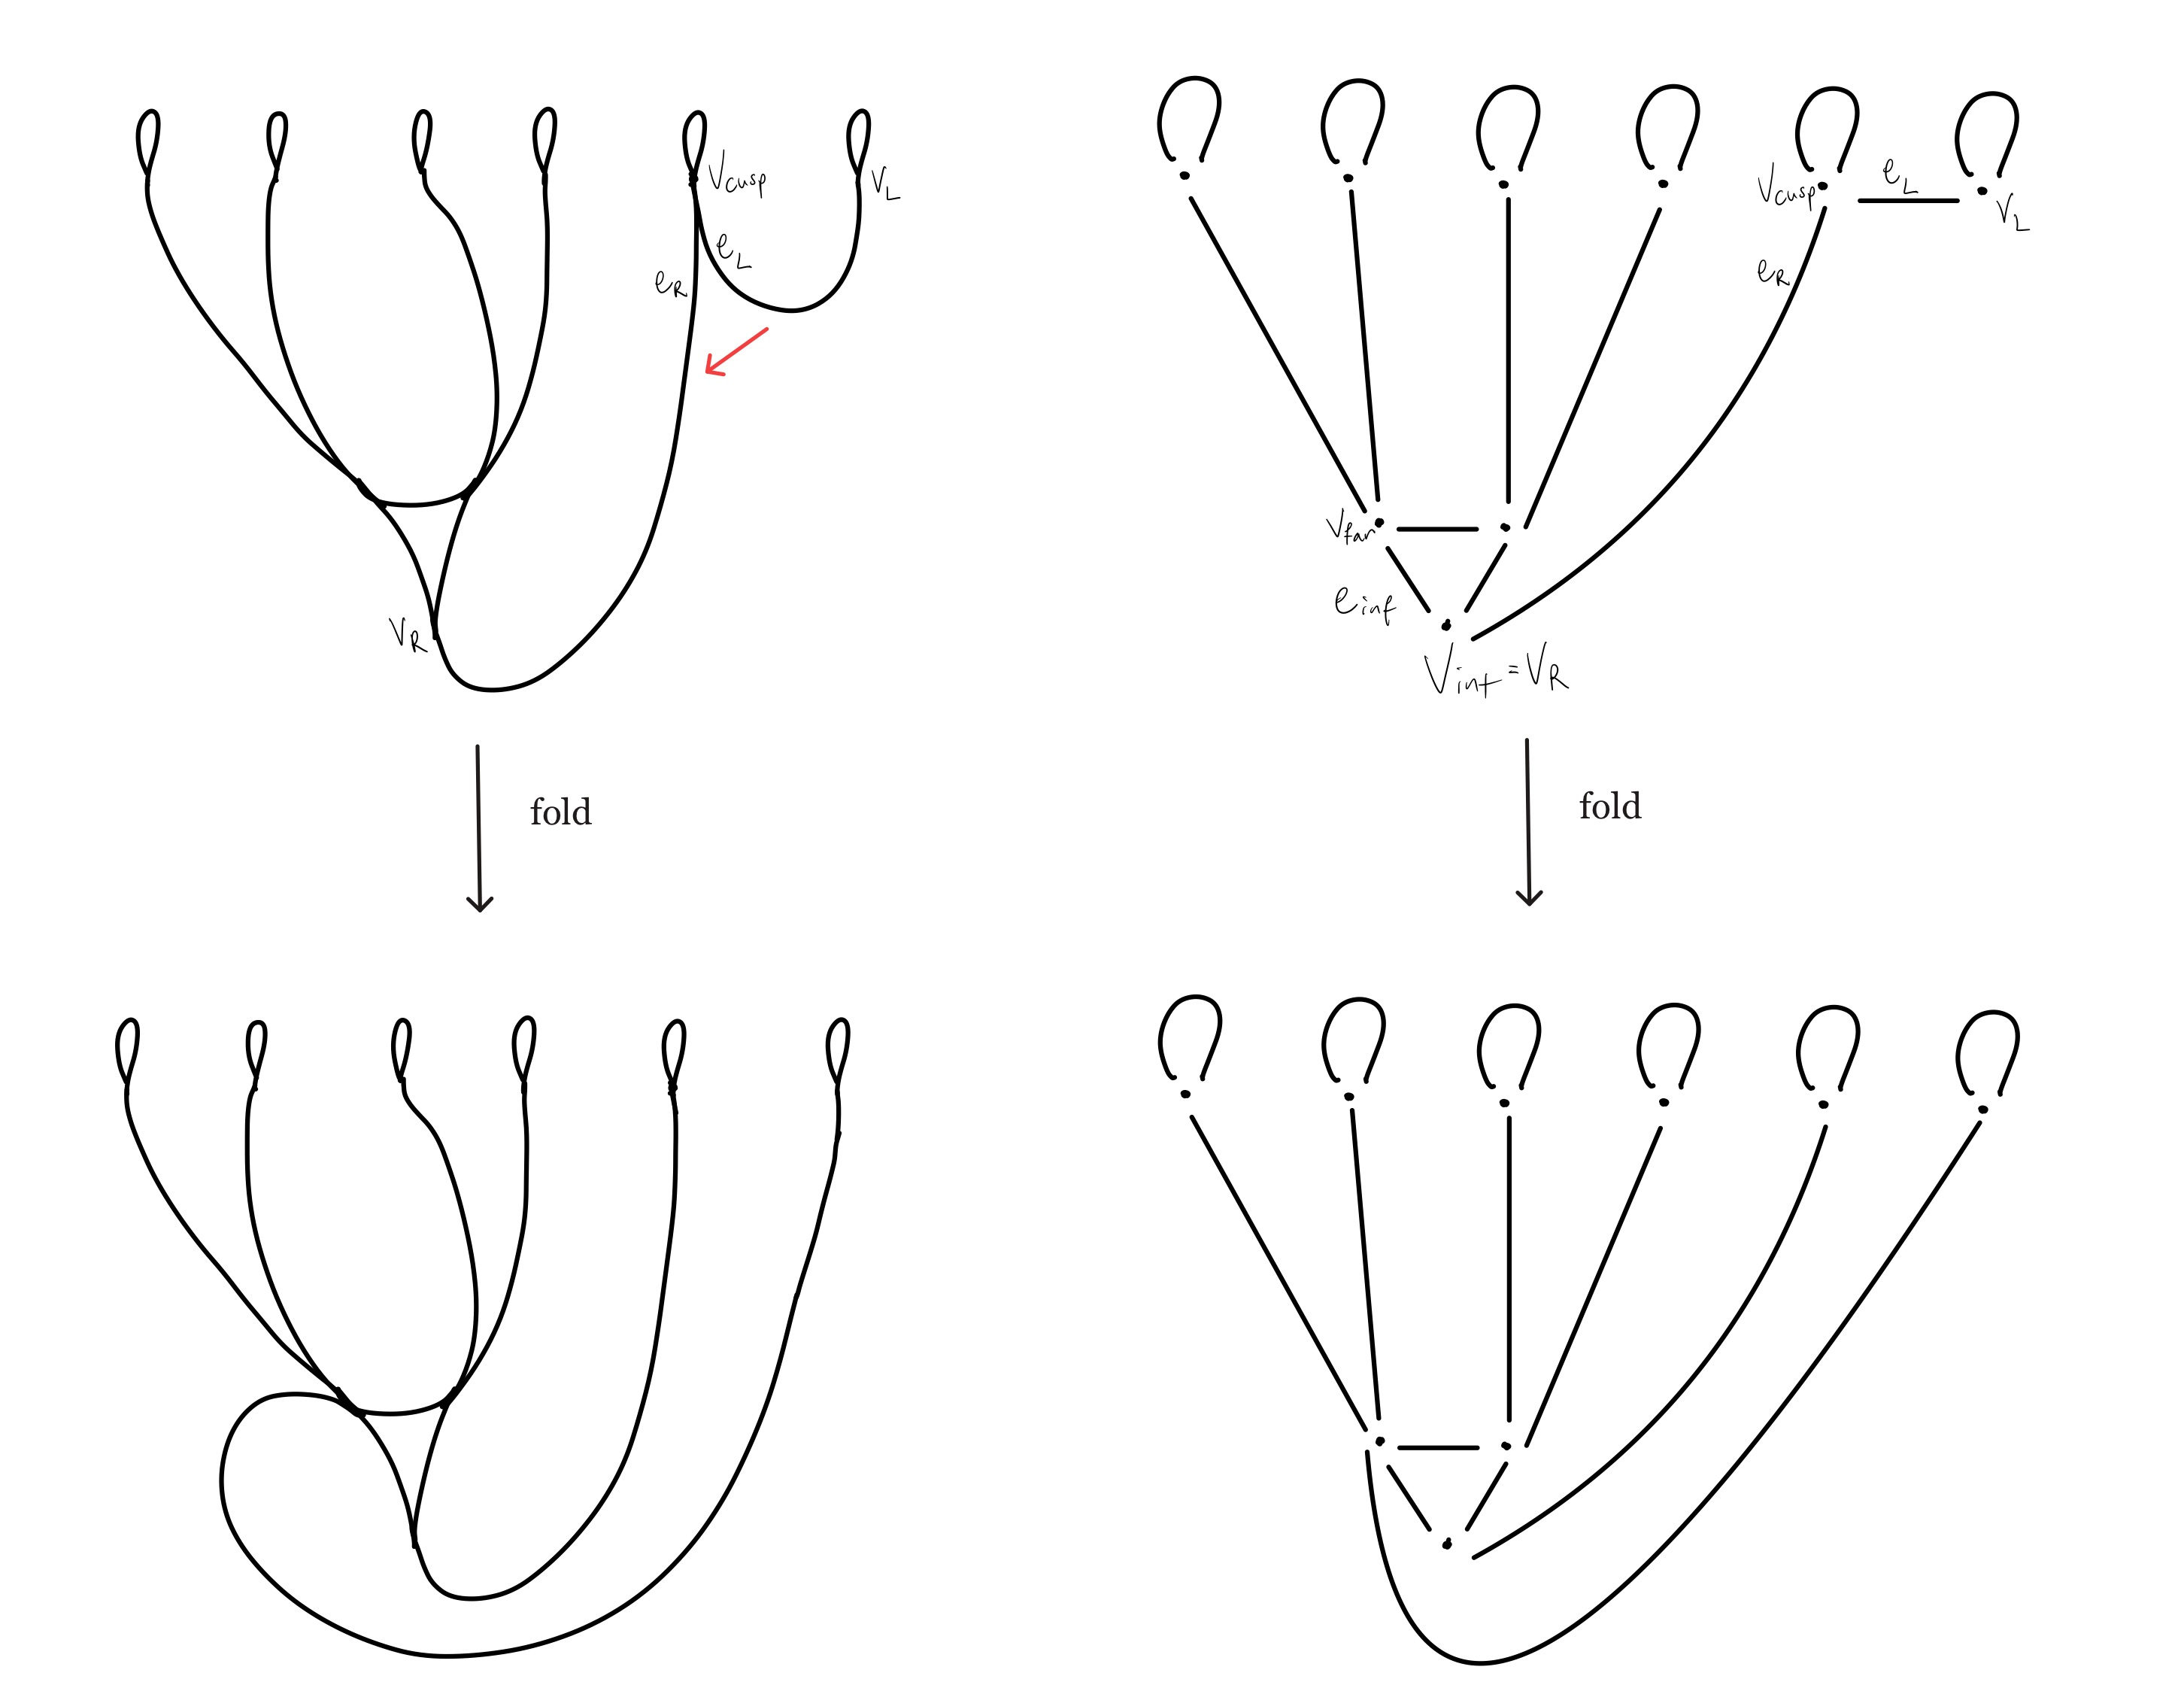
\includegraphics[width=\linewidth]{figures/Automaton Folding-1.jpg}
    \caption{Left: A left-to-right folding at the cusp located at $v_{cusp}$. Right: The equivalent operation performed by the algorithm on a \texttt{StandardTrainTrack} object. The algorithm deletes $e_L$, then attaches a new edge between $v_L$ and $v_{far}$ at the appropriate position in the cyclic ordering. The graph information, cyclic ordering, and cusp information are updated for the newly created \texttt{StandardTrainTrack} object.}
    \label{fig:folding_automaton}
\end{figure}

\subsection{Extended Automaton Capabilities}
\label{subsec:extended_capabilities}

A complete theoretical folding automaton encodes not only the set of standard train tracks (the vertices), but also the exact standardizing braids and transition matrices associated with the folding maps between them (the directed edges).

Our software package, \texttt{autofolder}, is fully equipped to compute this edge data. It features a robust standardization module that analyzes the global connectivity of a folded strand (identifying how it ``swings'' and ``winds'' around puncture clusters) to automatically derive the specific Artin braid generators required to return the track to standard form. Furthermore, it strictly tracks the permutation of real edges to compute the exact linear transition matrices induced on the space of transverse measures.

However, because the primary objective of this thesis is to classify pseudo-Anosov maps via manual topological case analysis and the Trace Lemma, we strictly require only the exhaustive list of candidate standard train tracks generated by the automaton. The complex cycle structure, explicit braid words, and transition matrices of the automaton's edges are not necessary for our obstruction. Consequently, we omit the dense algorithmic details of the standardization and matrix computations here, and focus our algorithm specifically on the Breadth-First Search mechanism used to exhaustively discover the state space (the vertices).

\subsection{The \texttt{autofolder} Enumeration Algorithm}

We now present the streamlined pseudo-code for our implementation, focused specifically on state enumeration. By leveraging the combinatorial equivalence checks detailed in Section \ref{subsec:comb_iso}, the algorithm efficiently generates the finite catalog of train tracks for any given stratum.

\begin{algorithm}[H]
\caption{autofolder: Train Track Enumeration}
\label{alg:autofolder_enum}
\begin{algorithmic}[1]
\Require An initial ``seed'' standard train track $\tau_{seed}$ belonging to stratum $\mathcal{S}$.
\Ensure The exhaustive list $L$ of all isomorphism classes of standard train tracks in $\mathcal{S}$.

\State $L \gets$ \textbf{List}($\{ \tau_{seed} \}$) \Comment{Ordered list of discovered isomorphism classes}
\State $Q \gets$ \textbf{Queue}($\{ \tau_{seed} \}$) \Comment{Queue for BFS exploration}

\While{$Q$ is not empty}
    \State $\tau_{curr} \gets \Call{Dequeue}{Q}$
    \State $\mathcal{K} \gets \tau_{curr}.\texttt{cusps}$

    \For{each cusp $c \in \mathcal{K}$}
        \For{each direction $d \in \{ \text{Right-over-Left}, \text{Left-over-Right} \}$}
            \State \Comment{1. Perform the combinatorial fold}
            \State $\tau_{folded} \gets \Call{Fold}{\tau_{curr}, c, d}$
            \If{$\tau_{folded}$ is Invalid} \textbf{continue} \EndIf

            \State \Comment{2. Linear Search for Isomorphism}
            \State $is\_new\_state \gets \textbf{True}$

            \For{$\tau_{ex} \in L$}
                \If{$\Call{IsIsomorphic}{\tau_{folded}, \tau_{ex}}$}
                    \State $is\_new\_state \gets \textbf{False}$
                    \State \textbf{break}
                \EndIf
            \EndFor

            \State \Comment{3. Record new tracks}
            \If{$is\_new\_state$}
                \State $\Call{Enqueue}{Q, \tau_{folded}}$
                \State $\Call{Append}{L, \tau_{folded}}$
            \EndIf
        \EndFor
    \EndFor
\EndWhile

\State \Return $L$
\end{algorithmic}
\end{algorithm}

%%%%%%%%%%%%%%%%%%%%%%%%%%%%%%%%%%%%%%%%%%%%%%%%%%%%%%%%%%%%%%%%%%%%%%%%%
%%% ARCHIVE: EXTENDED AUTOMATON CAPABILITIES (CODE)                   %%%
%%% Excluded from this dissertation by design (see                     %%%
%%% Section \ref{subsec:extended_capabilities}). May be enabled for   %%%
%%% follow-up papers covering the full graph implementation, including %%%
%%% standardizing braids and transition matrices.                      %%%
%%%%%%%%%%%%%%%%%%%%%%%%%%%%%%%%%%%%%%%%%%%%%%%%%%%%%%%%%%%%%%%%%%%%%%%%%
\iffalse

\subsection{Implementation of the Standardization Algorithm}
\label{subsec:standardization_implementation}

As established in Section \ref{subsec:standardizing_braid}, the train track $\tau'$ resulting from a fold is generally only \textit{almost standard}. While it remains a valid train track, it may violate the vertical marking condition required for our automaton's vertices. To resolve this, we must identify a \textit{standardizing braid} $\beta$ such that $\beta^{-1}(\tau')$ is standard.

The \texttt{standardizing} module implements this procedure in the function \texttt{standardizing\_braid}. Unlike the folding operation, which is purely local, standardization requires analyzing the global topology of the track relative to the vertical markings.

The algorithm proceeds in three phases:

\begin{enumerate}
    \item \textbf{Simulated Folding and State Analysis:}
    The function accepts the original standard track $\tau$ and the folding parameters (cusp and direction). It creates a temporary copy of $\tau$ and executes the combinatorial fold (as described in Section \ref{subsec:folding_implementation}).

    The algorithm then examines the local geometry of the \textit{far vertex} $v_{far}$ (the destination of the fold) in this new track. Specifically, it compares the position of the newly created real edge $e_{new}$ relative to the infinitesimal edge $e_{inf}$ that was traversed.
    \begin{itemize}
        \item \textbf{Swing Detection:} The algorithm checks the cyclic ordering $\mathcal{O}_{v_{far}}$. If $e_{new}$ is immediately counter-clockwise to $e_{inf}$, we classify this as a ``Swing Left''. If it is clockwise, it is a ``Swing Right''. This determines the local direction in which the strand has been pulled past the puncture.
    \end{itemize}

    \item \textbf{Global Connectivity Check (Wind Detection):}
    The ``Swing'' determines the local move, but to define the braid, we must determine how many punctures the strand crosses. This requires determining if the folded strand wraps around the puncture cluster to the left or the right.

    The algorithm computes the connected components of the graph $G' \setminus \{e_{new}\}$. By identifying which component contains specific marked points (relative to the linear ordering of punctures defined by the \texttt{side\_swapping\_edges}), the algorithm determines a ``Wind'' direction:
    \begin{itemize}
        \item \textbf{Wind Left:} The strand connects back to the rest of the track in a way that encloses punctures to the left of the active site.
        \item \textbf{Wind Right:} The strand encloses punctures to the right.
    \end{itemize}
    This step effectively implements a Breadth-First Search (BFS) on the graph components to detect obstructions to isotopy.

    \item \textbf{Braid Word Construction:}
    The combination of ``Swing'' and ``Wind'' directions uniquely determines the standardizing braid generator and its range. The algorithm calculates the range $[i, j]$ of punctures involved, where $i$ is the index of the folded puncture and $j$ is determined by the connectivity check (the ``landing spot'' of the strand).

    Based on the four possible geometric configurations, the software assigns the braid word:
    \begin{itemize}
        \item \textbf{Swing Left / Wind Right:} Corresponds to $\delta_{[i, j]}^{-1}$.
        \item \textbf{Swing Left / Wind Left:} Corresponds to $\delta_{[j, i]}$.
        \item \textbf{Swing Right / Wind Left:} Corresponds to $\delta_{[j, i]}$.
        \item \textbf{Swing Right / Wind Right:} Corresponds to $\delta_{[i, j]}^{-1}$.
    \end{itemize}
    Here, $\delta_{[i,j]}$ represents the standard Artin braid generator (or half-twist block) $\sigma_{j-1} \dots \sigma_i$.
\end{enumerate}

The function returns the braid string $\beta$. In the automaton construction, this string labels the edge, while the combinatorial isomorphism class of the folded track $\tau'$ serves as the destination vertex.

\subsection{Transition Matrices}
\label{subsec:transition_matrices}

A primary application of the folding automaton is the computation of the dilatation of pseudo-Anosov mapping classes. This dilatation $\lambda$ appears as the spectral radius of the transition matrix associated with the cycle in the automaton. Therefore, our software must rigorously compute and store the linear transformation induced by each fold on the space of transverse measures.

Let $V$ be the vector space spanned by the real edges of the train track. A fold transforms the set of real edges, inducing a linear map $M: V(\tau) \to V(\tau')$. Our implementation distinguishes between two cases:

\begin{enumerate}
    \item \textbf{Non-Isomorphic Transition (New State):}
    If the folded track $\tau'$ represents a new isomorphism class not yet in the automaton, the transition matrix is simply the \textit{elementary folding matrix} $E$.
    Geometrically, if a fold occurs at a cusp where branches $e_L$ and $e_R$ merge into a single branch, the weights transform as $w_{new} = w_L + w_R$. In the dual basis (lengths), this corresponds to an elementary matrix where one column is the sum of two others.
    The function \texttt{give\_edge\_label\_non\_isomorphic\_after\_folding} constructs this matrix by identifying the specific indices of the edges involved in the fold and applying the corresponding column operation to the identity matrix.

    \item \textbf{Isomorphic Transition (Closing a Cycle):}
    If the folded track $\tau'$ is combinatorially isomorphic to an existing state $\tau_{ex}$ in the automaton, we must account for the relabeling of edges. The transition is the composition of the folding map followed by the combinatorial isomorphism:
    \[
        \tau \xrightarrow{\text{fold}} \tau' \xrightarrow{\phi} \tau_{ex}
    \]
    The corresponding matrix is $M = P_\phi \cdot E$, where $P_\phi$ is the permutation matrix induced by the isomorphism $\phi: \tau' \to \tau_{ex}$.

    The function \texttt{transitionmatrix\_folding} implements this logic. As described in Section \ref{subsec:data_structures}, the algorithm first finds the explicit permutation of vertices and edges that realizes the isomorphism $\tau' \cong \tau_{ex}$. It then constructs $P_\phi$ by mapping the edge indices of $\tau'$ to the edge indices of $\tau_{ex}$. Finally, it applies the elementary folding operation to this permuted system, ensuring that the matrix correctly maps the edge weights of the source vertex $\tau$ to the edge weights of the canonical destination vertex $\tau_{ex}$.
\end{enumerate}

These matrices are stored as labels on the edges of the graph $\mathcal{A}$, allowing for the subsequent extraction of the cycle matrix by multiplying the matrices along any directed path.

\subsection{The Detailed \texttt{autofolder} Algorithm}
We now present the detailed pseudo-code for our full graph implementation. Unlike the theoretical model which assumes an $O(1)$ canonical form check, our implementation relies on a linear search through the discovered strata to handle the complexity of the braid group action. This formulation explicitly captures the mechanisms for managing the embedding data (side-swapping edges) and the isomorphism search used in our Python package.

\begin{algorithm}[p]
\caption{autofolder: Automaton Generation Implementation (Full Graph)}
\label{alg:autofolder_impl}
\begin{algorithmic}[1]
\Require An initial ``seed'' standard train track $\tau_{seed}$
\Ensure The Folding Automaton graph $\mathcal{A} = (V_{\mathcal{A}}, E_{\mathcal{A}})$

\State $L \gets$ \textbf{List}($\{ \tau_{seed} \}$) \Comment{Ordered list of discovered isomorphism classes}
\State $Q \gets$ \textbf{Queue}($\{ \tau_{seed} \}$) \Comment{Queue for BFS processing}
\State $E_{\mathcal{A}} \gets \emptyset$

\While{$Q$ is not empty}
    \State $\tau_{curr} \gets \Call{Dequeue}{Q}$
    \State $\mathcal{K} \gets \tau_{curr}.\texttt{cusps}$

    \For{each cusp $c \in \mathcal{K}$}
        \For{each direction $d \in \{ 0, 1 \}$ (Right-over-Left / Left-over-Right)}
            \State \Comment{1. Perform the combinatorial fold}
            \State $\tau_{folded} \gets \Call{Fold}{\tau_{curr}, c, d}$
            \If{$\tau_{folded}$ is Invalid} \textbf{continue} \EndIf

            \State \Comment{2. Compute Standardizing Braid}
            \State $\beta_{std} \gets \Call{StandardizingBraid}{\tau_{curr}, c, d}$

            \State \Comment{3. Update Embedding Data (Crucial Step)}
            \State \Comment{Apply braid permutation to vertical markers}
            \State $\tau_{folded}.\texttt{side\_swapping} \gets \Call{Action}{\beta_{std}, \tau_{folded}.\texttt{side\_swapping}}$

            \State \Comment{4. Linear Search for Isomorphism}
            \State $found \gets \textbf{False}$
            \State $idx_{target} \gets -1$

            \For{$\tau_{ex} \in L$}
                \If{$\Call{IsIsomorphic}{\tau_{folded}, \tau_{ex}}$}
                    \State $found \gets \textbf{True}$
                    \State $idx_{target} \gets \Call{Index}{L, \tau_{ex}}$
                    \State \Comment{Compute matrix with permutation}
                    \State $M_{trans} \gets \Call{TransitionMatrixFolding}{\tau_{folded}, \tau_{ex}, c, d}$
                    \State \textbf{break}
                \EndIf
            \EndFor

            \If{\textbf{not} $found$}
                \State \Comment{New state discovered}
                \State $\Call{Enqueue}{Q, \tau_{folded}}$
                \State $\Call{Append}{L, \tau_{folded}}$
                \State $idx_{target} \gets \Call{Size}{L} - 1$
                \State \Comment{Compute elementary folding matrix}
                \State $M_{trans} \gets \Call{MatrixNonIsomorphic}{\tau_{curr}, \tau_{folded}, c, d}$
            \EndIf

            \State \Comment{5. Add Edge to Automaton}
            \State $e \gets (\tau_{curr} \to L[idx_{target}])$
            \State $\text{Label}(e) \gets (\beta_{std}, M_{trans})$
            \State $E_{\mathcal{A}} \gets E_{\mathcal{A}} \cup \{e\}$
        \EndFor
    \EndFor
\EndWhile

\State \Return $(L, E_{\mathcal{A}})$
\end{algorithmic}
\end{algorithm}

\fi
%%%%%%%%%%%%%%%%%%%%%%%%%%%%%%%%%%%%%%%%%%%%%%%%%%%%%%%%%%%%%%%%%%%%%%%%%
%%% END OF ARCHIVE                                                    %%%
%%%%%%%%%%%%%%%%%%%%%%%%%%%%%%%%%%%%%%%%%%%%%%%%%%%%%%%%%%%%%%%%%%%%%%%%%


\section{Conclusion}

In this chapter, we formalized the theory of folding automata and provided a complete algorithmic realization of the enumeration framework originally theorized by Ko, Los, and Song \cite{SongEntropy}. As noted by Los \cite{Los2008}, a systematic study of all pseudo-Anosov homeomorphisms within a given stratum requires the rigorous development of its specific train-track automata theory. Furthermore, Los anticipated that because such automata are practically immense, an explicit algorithmic description is strictly necessary to make the state space tractable.

For the remaining non-orientable strata on the disk---specifically $(2; 1^6; 3^2)$ and $(3; 1^6; 3)$---our \texttt{autofolder} implementation fulfills this exact requirement. It provides a sufficient list of standard train tracks within each stratum, from which we can systematically hunt for valid train track maps.

However, executing this algorithmic enumeration reveals an immediate practical challenge: just as Los predicted, the raw topological output of the automaton is massive. The unrestricted state space contains a vast number of standard tracks, many of which possess localized, topologically redundant complexities known as \textit{joints}. Attempting to manually construct maps and apply the Trace Lemma across this entire, unpruned space would remain analytically intractable.

To bridge the gap between algorithmic enumeration and manual topological analysis, we apply, in Chapter \ref{chap:stratatraintrackanalysis}, the geometric operation of \textit{tight splitting}. By applying tight splitting to our enumerated tracks, we resolve these localized complexities and strictly reduce the automaton's massive output to a minimal, canonical set of jointless standard train tracks. It is upon this highly refined, manageable set of candidate tracks that our final Trace Lemma arguments are executed.